\chapter{Introducción}

Presentar de forma atractiva el trabajo... quizás renombrar el título del trabajo utilizando "all you need", como por ejemplo 

"All you need is sound and music: explorando la interacción creativa con modelos de lenguaje a gran escala en la creación sonora con lenguajes de programación musical"


\begin{figure}[H]
    \caption[Número de publicaciones de \textit{Deep Learning} por año que contienen la expresión <<all you need>> en el título]{Número de publicaciones de \textit{Deep Learning} por año que contienen la expresión <<all you need>> en el título.}
    \centering
    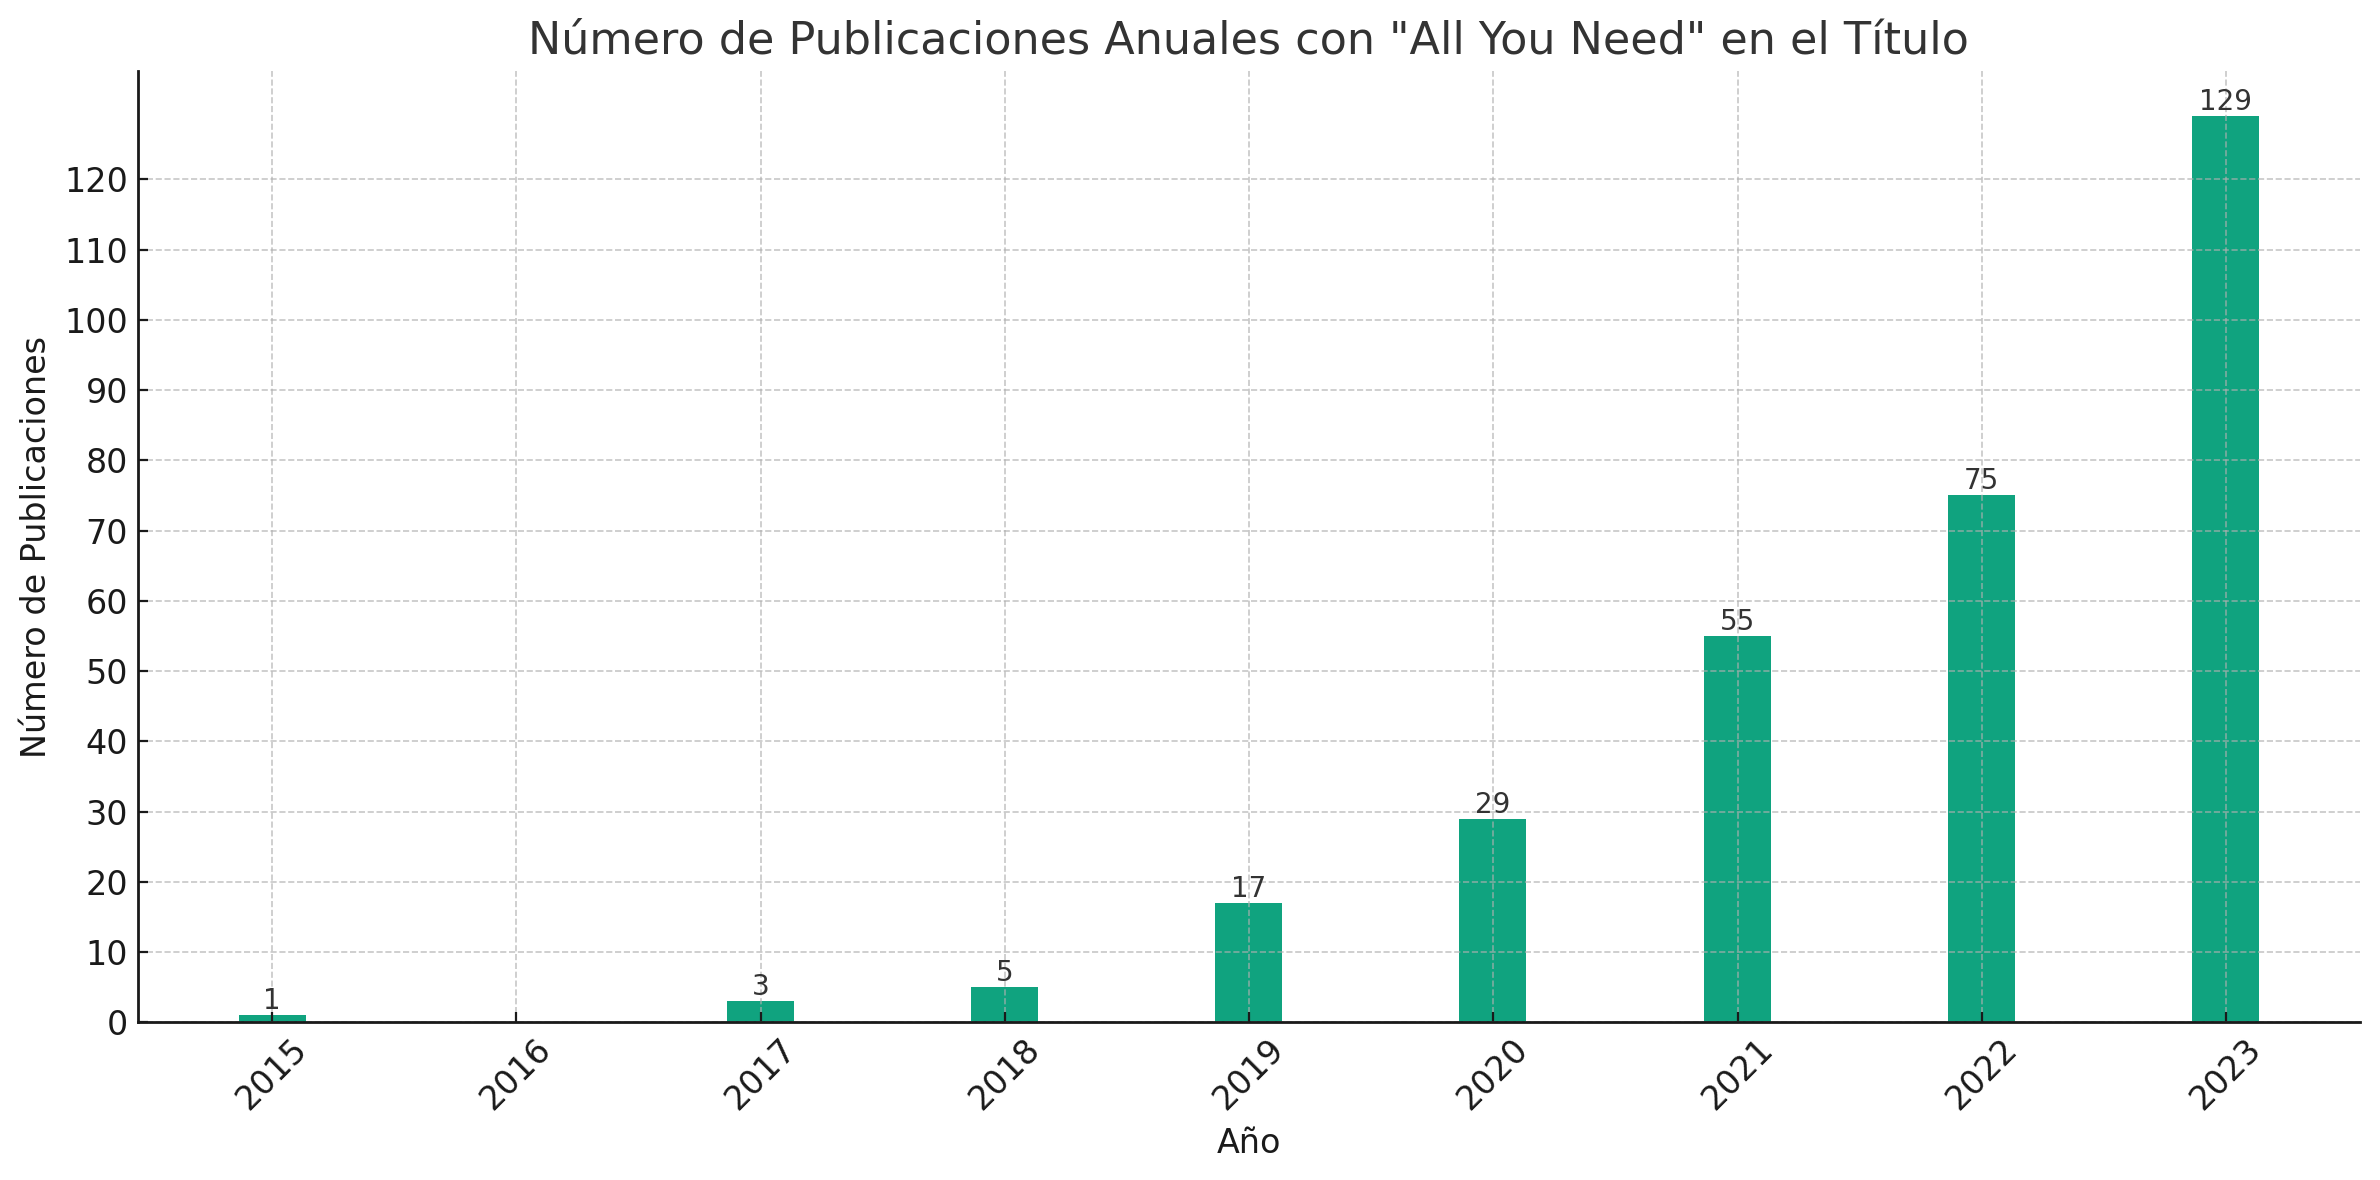
\includegraphics[width=0.9\textwidth]{./figuras/all_you_need_publicacionies_anuales.png}
    \source{Elaboración propia a partir del listado de \url{https://github.com/KentoNishi/awesome-all-you-need-papers}}
    \label{fig:all_you_need_publicaciones}
\end{figure}




